\documentclass[10pt,twocolumn,letterpaper]{article}

% ============================================================
%  IEEE-CONFERENCE-STYLE EMULATION
%  (IEEEtran.cls is not available in this build environment /
%   no network access to fetch it, so the standard IEEE
%   conference layout is reproduced with core LaTeX packages.)
% ============================================================
\usepackage[left=0.625in,right=0.625in,top=0.75in,bottom=1in,columnsep=0.22in]{geometry}
\usepackage{times}
\usepackage[T1]{fontenc}
\usepackage{graphicx}
\usepackage{amsmath,amssymb}
\usepackage{booktabs}
\usepackage{array}
\usepackage{caption}
\usepackage{enumitem}
\usepackage{microtype}
\usepackage[hidelinks]{hyperref}
\usepackage{titlesec}
\usepackage{authblk}[]{}
\usepackage{balance}
\usepackage{stfloats}

\usepackage{tikz}
\usetikzlibrary{shapes.geometric,arrows.meta,positioning,fit,calc,decorations.pathreplacing,backgrounds}
\usepackage{pgfplots}
\pgfplotsset{compat=1.18}

% ---------- IEEE-like caption style ----------
\captionsetup[figure]{font=footnotesize,labelfont={bf,footnotesize},labelsep=period,skip=4pt}
\captionsetup[table]{font=footnotesize,labelfont={bf,footnotesize},labelsep=period,skip=4pt}

% ---------- IEEE-like section headings ----------
% I. INTRODUCTION  (centered, small caps, bold)
\titleformat{\section}
  {\centering\normalfont\fontsize{10}{12}\bfseries\scshape}
  {\thesection.}{0.6em}{}
\titlespacing{\section}{0pt}{*2.2}{*1.3}

% A. Subsection Title  (run-in style, italic)
\titleformat{\subsection}[runin]
  {\normalfont\fontsize{10}{12}\itshape}
  {\thesubsection}{0.4em}{}[.\hspace{0.4em}]
\titlespacing{\subsection}{0pt}{*1.3}{0.6em}

\renewcommand{\thesection}{\Roman{section}}
\renewcommand{\thesubsection}{\Alph{subsection}}

% ---------- misc ----------
\setlength{\parindent}{1em}
\setlength{\parskip}{0pt}
\linespread{0.99}

% Avoid LaTeX vertically centering floats on float-only pages
% (figure* uses the double-column float registers, not the
%  single-column ones, so both must be set)
\makeatletter
\setlength{\@fptop}{0pt}
\setlength{\@fpbot}{0pt plus 1fil}
\setlength{\@dblfptop}{0pt}
\setlength{\@dblfpbot}{0pt plus 1fil}
\makeatother

% Allow a bottom float to share a page with only a small amount of
% text above it (needed so Fig. 4 can land on the same page as the
% tail of the reference list instead of being deferred to a new page).
\renewcommand{\textfraction}{0.03}
\renewcommand{\bottomfraction}{0.95}
\renewcommand{\topfraction}{0.95}
\renewcommand{\dbltopfraction}{0.95}
\renewcommand{\dblfloatpagefraction}{0.05}
\renewcommand{\floatpagefraction}{0.05}

\newcommand{\bx}{\mathbf{x}}
\newcommand{\bX}{\mathbf{X}}
\newcommand{\bY}{\mathbf{Y}}
\newcommand{\bF}{\mathbf{F}}
\newcommand{\bP}{\mathbf{P}}
\newcommand{\bh}{\mathbf{h}}
\newcommand{\br}{\mathbf{r}}
\newcommand{\by}{\mathbf{y}}
\newcommand{\bM}{\mathbf{M}}
\newcommand{\E}{\mathcal{E}}
\newcommand{\Hs}{\hat{\mathcal{H}}}
\newcommand{\reals}{\mathbb{R}}
\DeclareMathOperator*{\topk}{top\text{-}k}

% ---------- title block (IEEE conference style) ----------
\title{\vspace{-4mm}\fontsize{18}{20}\selectfont\bfseries
Spatially Dynamic Mixture-of-Experts for\\ Adverse-Weather Salient Object Detection}
\author{
\normalsize Anonymous Author(s)\\
\normalsize\itshape Affiliation withheld for blind review\\
\normalsize\ttfamily [Blind review]
}
\date{}

\begin{document}

\twocolumn[
  \begin{@twocolumnfalse}
    \maketitle
    \vspace{-6mm}
    \begin{center}
    \begin{minipage}{0.92\textwidth}
    \small
    \noindent\textbf{\textit{Abstract}\textemdash}
    Salient object detection (SOD) degrades under adverse weather.
    Existing approaches condition on explicit weather labels or apply mixture-of-experts (MoE) to image restoration rather than segmentation.
    We present SpatialMoE-SOD, routing individual spatial tokens to separate expert networks at three independent pyramid scales without using weather labels during training or inference.
    A depthwise convolutional router and MLP select top-$K{=}2$ experts from 8 per scale via true sparse dispatch.
    Per-token routing entropy is injected as an explicit feature channel into the cross-attention decoder via learnable additive fusion.
    On WXSOD, the model achieves MAE $0.0192$ on 1,500 synthetic test images spanning 9 weather categories and $0.0168$ on 554 real-world test images spanning 5 weather categories.

    \vspace{2mm}
    \noindent\textbf{\textit{Index Terms}\textemdash}
    salient object detection, mixture-of-experts, adverse weather, sparse routing, cross-attention decoder
    \end{minipage}
    \end{center}
    \vspace{4mm}
  \end{@twocolumnfalse}
]

\section{Introduction}

SOD identifies visually prominent regions as pixel-wise masks, but performance degrades under adverse weather.
Two strategies address this: (1)~weather-label-conditioned models---NIFM~\cite{nifm2025}---require metadata at inference; (2)~MoE for weather restoration---WM-MoE~\cite{wmmoe2023}---targets pixel regression, not segmentation.
To our knowledge, existing MoE-SOD methods primarily explore modality-, scale-, or task-level routing for multi-modal inputs rather than per-token routing for single-RGB SOD.
To our knowledge, no existing method combines (a)~spatial token-level routing, (b)~independent routing at multiple pyramid scales, and (c)~an SOD decoder informed by routing confidence, all without weather-specific supervision.
Our contributions:
\begin{enumerate}[leftmargin=*,nosep,label=\arabic*)]
  \item A token-level spatial router that assigns each token to top-$K{=}2$ experts from 8 per scale, using depthwise-convolutional context, noisy top-$K$ gating, and true sparse dispatch.
  \item Three independent routers at scales $1/4$, $1/8$, $1/16$, each with a separate expert pool.
  \item Routing entropy, normalized by $\log 2$ for $K{=}2$, is injected as an explicit decoder feature via learnable additive fusion.
\end{enumerate}

\section{Related Work}

\subsection{Adverse-Weather SOD}
NIFM~\cite{nifm2025} fuses noise indicators from explicit weather-type one-hot vectors.
WXSOD~\cite{wxsod2025} provides 14,945 images with per-image weather labels and synthetic/real-world test splits for weather-robust SOD.

\subsection{MoE for Weather Restoration}
WM-MoE~\cite{wmmoe2023} uses weather-aware routing for adverse-weather image restoration, whereas our method performs spatial token-level routing for single-RGB SOD without weather-specific supervision.
Existing MoE weather methods target pixel regression, not segmentation.

\subsection{MoE for SOD}
To our knowledge, existing MoE-SOD methods primarily explore modality-, scale-, or task-level routing for multi-modal inputs rather than per-token routing for single-RGB SOD.
V-MoE~\cite{v-moe2021} established token-level top-$K$ routing for classification.
Routing entropy has been explored for uncertainty estimation in MoE classifiers. We additionally inject it as an explicit decoder feature for dense prediction, although its isolated contribution has not been evaluated by an ablation.

\section{Method}

Fig.~\ref{fig:arch} illustrates the full architecture.
A shared PVTv2-B4 backbone extracts multi-scale features; three independent SpatialMoE layers process tokens at each scale; a cross-attention decoder fuses the results and produces dense predictions.
We detail each component below.

% ============================================================
%  FIGURE 1 -- ARCHITECTURE OVERVIEW  (left-to-right pipeline)
% ============================================================
\begin{figure*}[t]
\centering
\resizebox{\textwidth}{!}{%
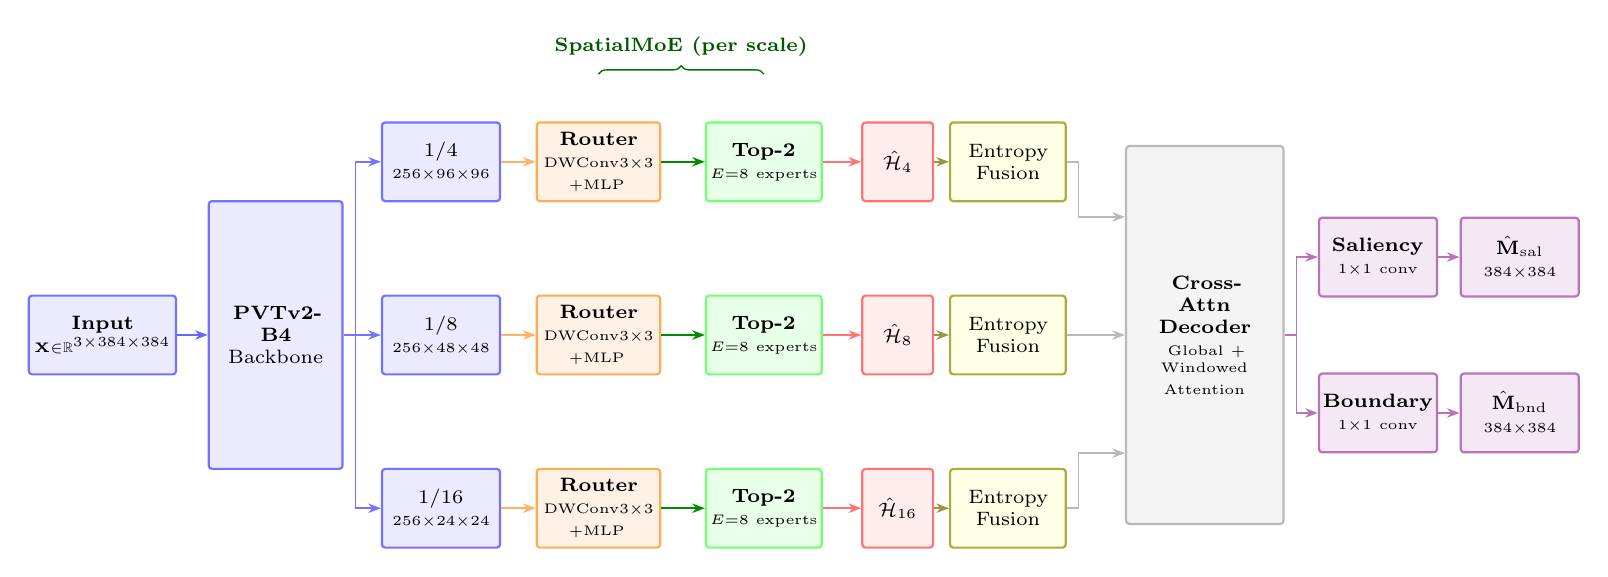
\begin{tikzpicture}[x=1mm,y=1mm,
  col_backbone/.style={fill=blue!8, draw=blue!55},
  col_router/.style={fill=orange!10, draw=orange!65},
  col_expert/.style={fill=green!9, draw=green!55},
  col_entropy/.style={fill=red!7, draw=red!55},
  col_merge/.style={fill=yellow!10, draw=yellow!65!black},
  col_decoder/.style={fill=gray!9, draw=gray!55},
  col_head/.style={fill=violet!9, draw=violet!55},
  col_scale/.style={font=\scriptsize\bfseries, text=blue!65!black},
  block/.style={rounded corners=1.2pt, draw, thick, minimum height=10mm, minimum width=15mm, align=center, font=\scriptsize, text width=14mm, inner sep=1pt},
  arr/.style={-{Stealth[length=1.6mm]}, line width=0.55pt, draw=black!65},
  carr/.style={-{Stealth[length=1.6mm]}, line width=0.55pt},
]

% --- column x-positions (mm) ---
\def\xIn{0}\def\xBb{20}\def\xSc{43}\def\xRt{63}\def\xEx{84}\def\xEn{101}\def\xFu{115}\def\xDe{140}\def\xHd{162}\def\xOu{180}
% --- row y-positions (mm) ---
\def\yTop{22}\def\yMid{0}\def\yBot{-22}

% === INPUT & BACKBONE (aligned with middle lane) ===
\node[block, col_backbone, minimum width=18mm, text width=18mm] (input) at (\xIn,\yMid) {\textbf{Input}\\ {\tiny$\bX{\in}\reals^{3\times384\times384}$}};
\node[block, col_backbone, minimum width=17mm, minimum height=34mm] (backbone) at (\xBb+2,\yMid) {\textbf{PVTv2-B4}\\ Backbone};

% === THREE PARALLEL LANES ===
\foreach \row/\y/\lbl/\dim in {top/\yTop/1/4/{256{\times}96{\times}96}, mid/\yMid/1/8/{256{\times}48{\times}48}, bot/\yBot/1/16/{256{\times}24{\times}24}}{}

% -- Lane: 1/4 (top) --
\node[block, col_backbone] (s4) at (\xSc,\yTop) {\scriptsize$1/4$\\ {\tiny$256{\times}96{\times}96$}};
\node[block, col_router, text width=15mm] (r4) at (\xRt,\yTop) {\textbf{Router}\\ {\tiny DWConv$3{\times}3$}\\ {\tiny +MLP}};
\node[block, col_expert, minimum width=13mm] (e4) at (\xEx,\yTop) {\textbf{Top-2}\\ {\tiny$E{=}8$ experts}};
\node[block, col_entropy, minimum width=9mm, text width=8mm] (h4) at (\xEn,\yTop) {$\Hs_4$};
\node[block, col_merge, minimum width=11mm] (ef4) at (\xFu,\yTop) {\scriptsize Entropy\\ Fusion};

% -- Lane: 1/8 (middle) --
\node[block, col_backbone] (s8) at (\xSc,\yMid) {\scriptsize$1/8$\\ {\tiny$256{\times}48{\times}48$}};
\node[block, col_router, text width=15mm] (r8) at (\xRt,\yMid) {\textbf{Router}\\ {\tiny DWConv$3{\times}3$}\\ {\tiny +MLP}};
\node[block, col_expert, minimum width=13mm] (e8) at (\xEx,\yMid) {\textbf{Top-2}\\ {\tiny$E{=}8$ experts}};
\node[block, col_entropy, minimum width=9mm, text width=8mm] (h8) at (\xEn,\yMid) {$\Hs_8$};
\node[block, col_merge, minimum width=11mm] (ef8) at (\xFu,\yMid) {\scriptsize Entropy\\ Fusion};

% -- Lane: 1/16 (bottom) --
\node[block, col_backbone] (s16) at (\xSc,\yBot) {\scriptsize$1/16$\\ {\tiny$256{\times}24{\times}24$}};
\node[block, col_router, text width=15mm] (r16) at (\xRt,\yBot) {\textbf{Router}\\ {\tiny DWConv$3{\times}3$}\\ {\tiny +MLP}};
\node[block, col_expert, minimum width=13mm] (e16) at (\xEx,\yBot) {\textbf{Top-2}\\ {\tiny$E{=}8$ experts}};
\node[block, col_entropy, minimum width=9mm, text width=8mm] (h16) at (\xEn,\yBot) {$\Hs_{16}$};
\node[block, col_merge, minimum width=11mm] (ef16) at (\xFu,\yBot) {\scriptsize Entropy\\ Fusion};

% === DECODER (spans all three lanes) ===
\node[block, col_decoder, minimum width=20mm, minimum height=48mm] (decoder) at (\xDe,\yMid) {\textbf{Cross-Attn}\\ \textbf{Decoder}\\[2pt] {\tiny Global + Windowed\\ Attention}};

% === OUTPUT HEADS ===
\node[block, col_head, minimum width=15mm] (sal) at (\xHd,\yTop*0.45) {\textbf{Saliency}\\ {\tiny$1{\times}1$ conv}};
\node[block, col_head, minimum width=15mm] (bnd) at (\xHd,\yBot*0.45) {\textbf{Boundary}\\ {\tiny$1{\times}1$ conv}};

% === FINAL OUTPUTS ===
\node[block, col_head, minimum width=15mm] (outsal) at (\xOu,\yTop*0.45) {$\hat{\bM}_{\text{sal}}$\\ {\tiny$384{\times}384$}};
\node[block, col_head, minimum width=15mm] (outbnd) at (\xOu,\yBot*0.45) {$\hat{\bM}_{\text{bnd}}$\\ {\tiny$384{\times}384$}};

% === ARROWS: Input -> Backbone ===
\draw[carr, draw=blue!60] (input) -- (backbone);

% === ARROWS: Backbone -> three lanes ===
% A short lead-out (\dOut) clears the arrow from the backbone box's own
% right border before it turns vertical -- with no lead-out at all the
% vertical run sat exactly on top of the box edge and read as part of
% the box outline. The remaining run into each lane box is still close
% to the straight middle arrow's length, since \dOut is kept small.
\def\dOut{1.5}
\draw[carr, draw=blue!55] (backbone.east) -- ++(\dOut,0) |- (s4.west);
\draw[carr, draw=blue!55] (backbone.east) -- (s8.west);
\draw[carr, draw=blue!55] (backbone.east) -- ++(\dOut,0) |- (s16.west);

% === ARROWS: per-lane pipeline ===
\foreach \s/\r/\e/\h/\ef in {s4/r4/e4/h4/ef4, s8/r8/e8/h8/ef8, s16/r16/e16/h16/ef16}{
  \draw[carr, draw=orange!60] (\s) -- (\r);
  \draw[carr, draw=green!55!black] (\r) -- (\e);
  \draw[carr, draw=red!55] (\e) -- (\h);
  \draw[carr, draw=yellow!55!black] (\h) -- (\ef);
}

% === ARROWS: Entropy Fusion -> Decoder ===
% Same lead-out fix as above -- gives a visible stub leaving each
% Entropy Fusion box (previously the bend sat right at the box edge,
% i.e. no stub at all) while the remaining run into the decoder stays
% close in length to the straight middle arrow.
\draw[carr, draw=gray!55] (ef4.east) -- ++(\dOut,0) |- ([yshift=15mm]decoder.west);
\draw[carr, draw=gray!55] (ef8.east) -- (decoder.west);
\draw[carr, draw=gray!55] (ef16.east) -- ++(\dOut,0) |- ([yshift=-15mm]decoder.west);

% === ARROWS: Decoder -> Heads ===
\draw[carr, draw=violet!55] (decoder.east) -- ++(\dOut,0) |- (sal.west);
\draw[carr, draw=violet!55] (decoder.east) -- ++(\dOut,0) |- (bnd.west);

% === ARROWS: Heads -> Outputs ===
\draw[carr, draw=violet!55] (sal) -- (outsal);
\draw[carr, draw=violet!55] (bnd) -- (outbnd);

% === Bracket label for SpatialMoE block (per lane) ===
\draw[decorate, decoration={brace, amplitude=3pt}, green!45!black, line width=0.5pt]
  ([yshift=6mm]r4.north) -- ([yshift=6mm]e4.north)
  node[midway, above=1mm, font=\scriptsize\bfseries, text=green!35!black] {SpatialMoE (per scale)};

\end{tikzpicture}%
}
\caption{\textbf{SpatialMoE-SOD architecture.}
Input $\bX \in \reals^{3 \times 384 \times 384}$ is processed by a PVTv2-B4 backbone to produce multi-scale features at $1/4$, $1/8$, $1/16$ resolution.
Each scale is independently processed by a SpatialMoE layer: a depthwise convolutional router selects top-$K{=}2$ experts from 8 via noisy gating, and a per-token entropy map $\Hs$ is computed.
The decoder merges scales via global and windowed cross-attention, with entropy features injected via learned additive fusion at each scale.
Two $1{\times}1$ conv heads produce saliency and boundary logits at full resolution.}
\label{fig:arch}
\end{figure*}

\subsection{Multi-Scale Features}
A PVTv2-B4 backbone~\cite{pvtv2} pretrained on ImageNet extracts features at three scales via $\texttt{out\_indices}=(0,1,2)$.
Each scale is projected to $C{=}256$ via $1{\times}1$ convolution:
\begin{equation}
  \bX_s = \text{Proj}_s(\text{Backbone}(\bX)_s) \in \reals^{C \times H_s \times W_s},
\end{equation}
where $s \in \{4, 8, 16\}$ with $(H_s,W_s) \in \{(96,96),(48,48),(24,24)\}$.
Each feature map is reshaped into $N_s = H_s \times W_s$ tokens $\bx_i \in \reals^C$.

\subsection{Router}
For each scale, a depthwise $3{\times}3$ convolution captures local spatial context from the feature map.
The router input concatenates each token with its local context:
\begin{equation}
  \br_i = [\bx_i \;|\; \text{DWConv}_{3\times3}(\bX_s)_i] \in \reals^{2C},
\end{equation}
where $|$ denotes channel-wise concatenation, yielding a $2C$-dimensional vector that encodes both the token's content and its spatial neighborhood.
A two-layer MLP produces routing logits:
\begin{equation}
  \bh_i = W_2 \cdot \text{GELU}(W_1 \br_i + b_1) + b_2 \in \reals^{E},
\end{equation}
with $W_1 \in \reals^{128 \times 2C}$, $W_2 \in \reals^{E \times 128}$, $E{=}8$ experts.
The hidden dimension 128 provides a bottleneck between the $2C{=}512$ input and $E{=}8$ output.

% ============================================================
%  FIGURE 2 -- ROUTING MECHANISM  (two-row / boustrophedon
%  layout: row 1 left-to-right, row 2 right-to-left, so the
%  diagram uses vertical space instead of squeezing everything
%  into one long horizontal strip)
% ============================================================
\begin{figure*}[t]
\centering
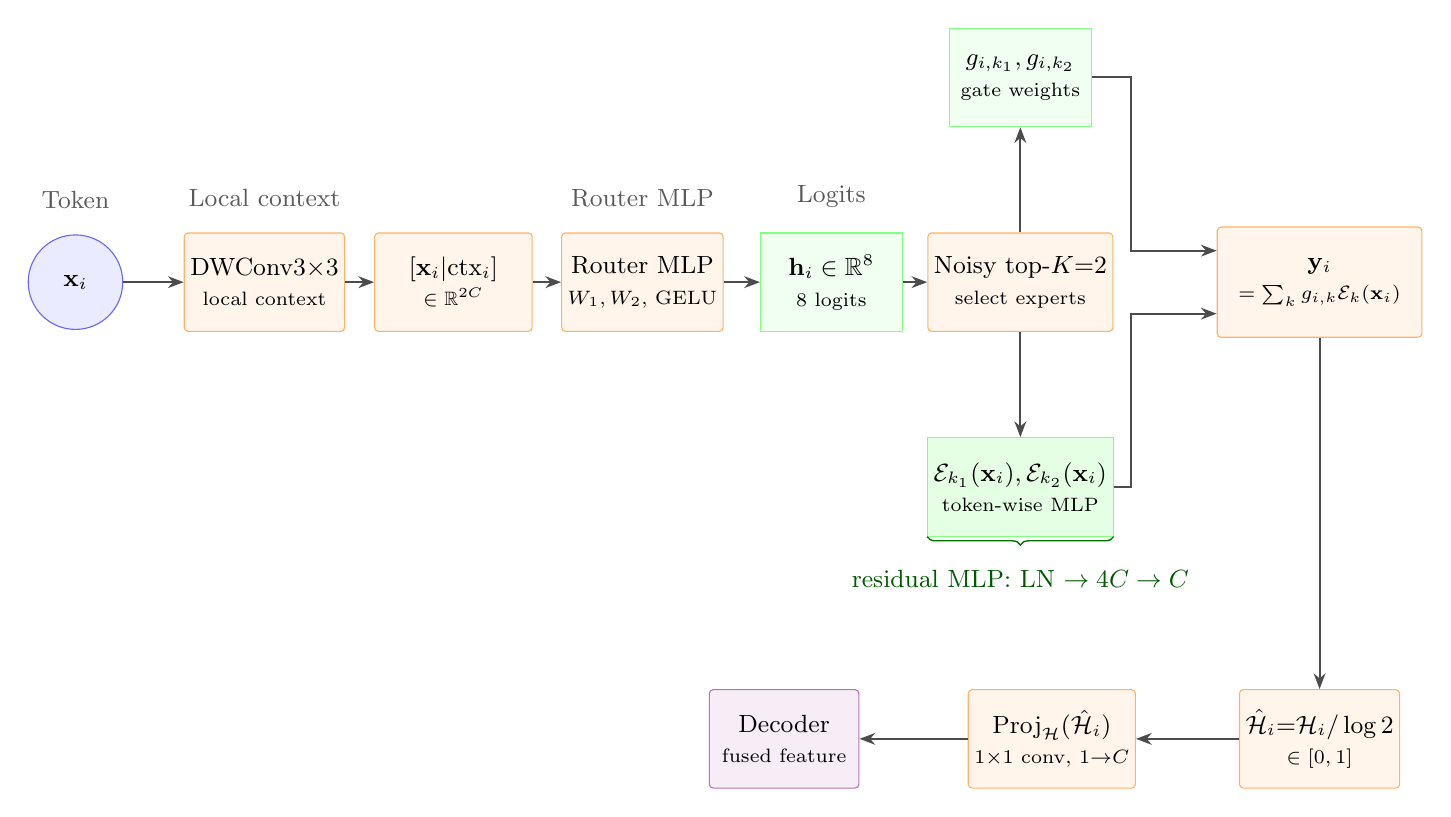
\begin{tikzpicture}[x=1mm,y=1mm,
  token/.style={circle, draw=blue!60, fill=blue!8, minimum size=12mm, font=\small\bfseries, inner sep=0pt},
  op/.style={rectangle, rounded corners=1.4pt, draw=orange!60, fill=orange!8, minimum height=12.5mm, minimum width=20mm, align=center, font=\small, inner sep=2.2pt},
  logits/.style={rectangle, draw=green!50, fill=green!6, minimum height=12.5mm, minimum width=18mm, align=center, font=\small, inner sep=2.2pt},
  expertnode/.style={rectangle, draw=green!50, fill=green!10, minimum height=12.5mm, minimum width=22mm, align=center, font=\small, inner sep=2.2pt},
  decnode/.style={rectangle, rounded corners=1.4pt, draw=violet!55, fill=violet!7, minimum height=12.5mm, minimum width=19mm, align=center, font=\small, inner sep=2.2pt},
  lbl/.style={font=\small, text=black!65},
  carr/.style={-{Stealth[length=2mm]}, line width=0.7pt, draw=black!70},
]

% --- Row 1 (top spine, left to right): token through the top-K
%     merge back into y_i. This half of the diagram is a single
%     spine with a small up/down branch, same as before -- no
%     long lines cross it, so nothing can collide with the label.
\def\yRowA{0}
\def\xTok{0}\def\xCtx{24}\def\xCat{48}\def\xMlp{72}\def\xLog{96}\def\xTopk{120}
\def\xBrE{120}\def\xSum{158}
\def\yBr{26}

\node[token] (xi) at (\xTok,\yRowA) {$\bx_i$};
\node[op] (local) at (\xCtx,\yRowA) {DWConv$3{\times}3$\\ {\scriptsize local context}};
\node[op] (concat) at (\xCat,\yRowA) {$[\bx_i | \text{ctx}_i]$\\ {\scriptsize $\in\reals^{2C}$}};
\node[op] (mlp) at (\xMlp,\yRowA) {Router MLP\\ {\scriptsize $W_1,W_2$, GELU}};
\node[logits] (logits) at (\xLog,\yRowA) {$\bh_i \in \reals^{8}$\\ {\scriptsize 8 logits}};
\node[op] (topk) at (\xTopk,\yRowA) {Noisy top-$K{=}2$\\ {\scriptsize select experts}};

% branch nodes sit directly above/below top-K, sharing its x so both
% branch arrows are plain straight verticals; the shared column also
% keeps a wide, unambiguous margin before the sum box.
\node[logits] (gate) at (\xBrE,\yBr) {$g_{i,k_1}, g_{i,k_2}$\\ {\scriptsize gate weights}};
\node[expertnode] (experts) at (\xBrE,-\yBr) {$\E_{k_1}(\bx_i), \E_{k_2}(\bx_i)$\\ {\scriptsize token-wise MLP}};

\node[op, minimum width=26mm, minimum height=14mm] (sum) at (\xSum,\yRowA) {$\by_i$\\ {\scriptsize$=\sum_k g_{i,k}\E_k(\bx_i)$}};

% --- Row 2 (bottom spine, right to left, directly below sum --
%     this half only starts once the top-K branch has already
%     merged, so it never has to cross the branch region at all) ---
\def\yRowB{-58}
\node[op] (entropy) at (\xSum,\yRowB) {$\Hs_i {=} \mathcal{H}_i/\log 2$\\ {\scriptsize $\in[0,1]$}};
\node[op] (proj) at (124,\yRowB) {$\text{Proj}_\mathcal{H}(\Hs_i)$\\ {\scriptsize $1{\times}1$ conv, $1{\to}C$}};
\node[decnode] (dec) at (90,\yRowB) {Decoder\\ {\scriptsize fused feature}};

% --- arrows: Row 1 spine ---
\draw[carr] (xi) -- (local);
\draw[carr] (local) -- (concat);
\draw[carr] (concat) -- (mlp);
\draw[carr] (mlp) -- (logits);
\draw[carr] (logits) -- (topk);

% --- arrows: branch out of top-K (plain straight verticals, since
%     gate/experts now share top-K's x-coordinate) ---
\draw[carr] (topk.north) -- (gate.south);
\draw[carr] (topk.south) -- (experts.north);

% --- arrows: branch back into sum (clean right-angle, entering
%     perpendicular to the box's west face -- vertical bend first,
%     then a straight horizontal run directly into the box edge,
%     offset above/below center so the two arrows don't overlap).
%     The shared branch column gives both a long, unambiguous
%     horizontal run instead of hugging the sum box. ---
% Both stubs bend at the SAME x-coordinate (\xStub), not at a fixed
% offset from each box's .east -- since gate (18mm wide) and experts
% (22mm wide) have different widths, ++(8,0) from .east previously put
% their elbows at different x positions, so the two arrows into sum.west
% were not parallel/aligned. Using an absolute x for the bend fixes this.
% \xStub is pulled back well clear of sum.west (was 143, only 2mm shy of
% sum.west at 145) so the two horizontal runs into the box are long
% enough to read as parallel lines instead of crowding into one point;
% the entry yshift is also widened (2mm->4mm) so the two arrowheads land
% clearly apart on the box edge instead of nearly touching.
\def\xStub{134}
\draw[carr] (gate.east) -- (\xStub,\yBr) |- ([yshift=4mm]sum.west);
\draw[carr] (experts.east) -- (\xStub,-\yBr) |- ([yshift=-4mm]sum.west);

% --- arrow: drop straight down from sum into Row 2 (clear of the
%     branch region entirely, so nothing to collide with) ---
\draw[carr] (sum.south) -- (entropy.north);

% --- arrows: Row 2 spine (right to left) ---
\draw[carr] (entropy.west) -- (proj.east);
\draw[carr] (proj.west) -- (dec.east);

% --- brace + caption for expert computation, directly under the experts box ---
\draw[decorate, decoration={brace, amplitude=3pt, mirror}, green!45!black, line width=0.5pt]
  (experts.south west) -- (experts.south east);
\node[lbl, below=3mm of experts, align=center, text=green!35!black] {residual MLP: LN $\to 4C \to C$};

% --- top labels (kept clear of the vertical branch arrows) ---
\node[lbl, above=2mm of xi] {Token};
\node[lbl, above=2mm of local] {Local context};
\node[lbl, above=2mm of mlp] {Router MLP};
\node[lbl, above=2mm of logits] {Logits};

\end{tikzpicture}
\caption{\textbf{Routing mechanism for token $\bx_i$ at one pyramid scale.}
A depthwise $3{\times}3$ convolution extracts local spatial context; the concatenation $\br_i = [\bx_i | \text{ctx}_i] \in \reals^{2C}$ is passed through a two-layer MLP to produce 8 routing logits.
Noisy top-$K{=}2$ selection (Gaussian noise during training) picks two experts, branching into gate weights (top) and expert outputs (bottom); gate weights are softmax over selected logits only.
The selected experts process the token independently; their outputs are summed with gate weights.
Routing entropy $\Hs_i \in [0,1]$ measures assignment uncertainty and is injected as a feature channel into the decoder via a learned $1{\times}1$ projection.}
\label{fig:router}
\end{figure*}


\subsection{Noisy Top-$K$ Routing}
During training, Gaussian noise is added with input-dependent scale to encourage exploration:
\begin{equation}
  \tilde{h}_{i,j} = h_{i,j} + \epsilon_{i,j}, \quad \epsilon_{i,j} \sim \mathcal{N}(0, \sigma_j^2(\bx_i)),
\end{equation}
where $\sigma_j(\bx_i) = \text{softplus}(w_j^\top \bx_i + b_j)$ is a learned per-expert, per-token noise scale.
At inference, noise is disabled ($\epsilon{=}0$).
Top-$K{=}2$ experts are selected per token; gate weights are softmax over selected logits only:
\begin{equation}
  g_{i,k} = \frac{\exp(\tilde{h}_{i,k})}{\sum_{j \in \mathcal{T}_i} \exp(\tilde{h}_{i,j})}, \quad k \in \mathcal{T}_i = \topk_j(\tilde{h}_{i,j}, K{=}2).
\end{equation}
This produces a sparse assignment: each token attends to exactly 2 of 8 experts, and each expert processes only the tokens that selected it.

\subsection{Sparse Expert Aggregation}
Each expert $\E_k$ executes only on tokens that selected it.
For expert $k$, let $\mathcal{A}_k = \{i : k \in \mathcal{T}_i\}$ denote its assigned tokens:
\begin{equation}
  \by_i = \sum_{k \in \mathcal{T}_i} g_{i,k} \cdot \E_k(\bx_i),
\end{equation}
implemented via a loop over experts with mask-based selection (true sparsity, not dense with masking).
Each expert is a token-wise residual MLP:
\begin{equation}
  \E_k(\bx) = \bx + W_k^{(2)} \cdot \text{GELU}(W_k^{(1)} \cdot \text{LN}(\bx)),
\end{equation}
with $W_k^{(1)} \in \reals^{4C \times C}$, $W_k^{(2)} \in \reals^{C \times 4C}$ ($4{\times}$ expansion from $C{=}256$ to $4C{=}1024$).
Each scale has 8 independent experts with no weight sharing (24 total).
Reshaping per-token outputs yields $\bY_s \in \reals^{C \times H_s \times W_s}$.

\subsection{Routing Entropy}
Per-token routing entropy measures assignment uncertainty over the selected experts:
\begin{equation}
  \mathcal{H}_i = -\sum_{k \in \mathcal{T}_i} g_{i,k} \log g_{i,k}, \quad \Hs_i = \mathcal{H}_i / \log 2 \in [0, 1].
\end{equation}
Division by $\log 2$ normalizes to $[0,1]$, where 0 indicates a single expert dominates and 1 indicates uniform assignment.
The normalized entropy map $\Hs_s \in \reals^{1 \times H_s \times W_s}$ is fused with MoE output via a learned additive block:
\begin{equation}
  \bF_s = \text{Proj}_Y(\bY_s) + \lambda_s \cdot \text{Proj}_\mathcal{H}(\Hs_s),
\end{equation}
where $\text{Proj}_\mathcal{H}$ is a $1{\times}1$ convolution from 1 to $C$ channels and $\lambda_s$ is a learnable scalar initialized to 0.1.
This allows the decoder to condition its attention on routing confidence without requiring the entropy to be differentiable through the expert weights.

\subsection{Decoder}
The decoder merges coarse-to-fine features via top-down cross-attention.
At the coarsest scale, $\bF_{16}$ is upsampled and used as queries with $\bF_8$ as keys and values (8-head global attention):
\begin{equation}
  \bF_8' = \text{GlobalCrossAttn}(Q = \text{Up}(\bF_{16}),\; KV = \bF_8).
\end{equation}
Global context is then injected into the fine scale: $\bF_4^{\text{ctx}} = \bF_4 + \text{Proj}_g(\text{AvgPool}(\bF_8'))$.
$\bF_8'$ is upsampled and used as queries with $\bF_4^{\text{ctx}}$ as keys and values using $7{\times}7$ windowed attention for efficiency:
\begin{equation}
  \bF_4' = \text{WinCrossAttn}(Q = \text{Up}(\bF_8'),\; KV = \bF_4^{\text{ctx}}).
\end{equation}
Three refinement blocks (each: Conv $3{\times}3$ $\to$ GroupNorm $\to$ ReLU $\to$ Conv $3{\times}3$ $\to$ GroupNorm $\to$ ReLU $\to$ residual addition) progressively upsample from $1/4$ to full resolution.
Two $1{\times}1$ convolution heads produce saliency logits $\hat{\bM}_{\text{sal}}$ and boundary logits $\hat{\bM}_{\text{bnd}}$ at $384{\times}384$.

\subsection{Training Objective}
The total loss combines four active terms (all other terms in the codebase are inactive):
\begin{equation}
  \mathcal{L} = \mathcal{L}_{\text{BCE}} + \lambda_{\text{IoU}}\mathcal{L}_{\text{IoU}} + \lambda_{\text{LB}}\mathcal{L}_{\text{LB}} + \lambda_{\text{IMP}}\mathcal{L}_{\text{IMP}},
\end{equation}
with $\lambda_{\text{IoU}}{=}1.0$, $\lambda_{\text{LB}}{=}\lambda_{\text{IMP}}{=}0.01$.
$\mathcal{L}_{\text{BCE}}$ is binary cross-entropy with logits between predicted saliency logits and ground-truth mask.
$\mathcal{L}_{\text{IoU}}$ is the soft IoU loss:
$1 - \text{mean}_b\!\left[\frac{\sum_{hw}\sigma(\hat{M}_b) \cdot M_b + \epsilon}{\sum_{hw}\sigma(\hat{M}_b) + \sum_{hw} M_b - \sum_{hw}\sigma(\hat{M}_b) \cdot M_b + \epsilon}\right]$.
$\mathcal{L}_{\text{LB}}$ is the load-balancing loss:
$\frac{1}{|\mathcal{S}|}\sum_{s} E \sum_j f_j^{(s)} P_j^{(s)}$, where $f_j$ is the fraction of all routing slots assigned to expert $j$, computed from hard assignments and detached, and $P_j$ is the differentiable mean gate mass.
$\mathcal{L}_{\text{IMP}}$ is the importance loss:
$\frac{1}{|\mathcal{S}|}\sum_{s} (\text{std}(\bP^{(s)}) / \text{mean}(\bP^{(s)}))^2$, where $\bP^{(s)} \in \reals^E$ denotes the per-expert mean gate-mass vector at scale $s$.
Deep supervision, boundary, and SSIM losses are defined in the codebase but inactive in the reported configuration; deep supervision is disabled at the model level, while the boundary and SSIM loss weights are zero.

\section{Experiments}

\subsection{Setup}
We evaluate on WXSOD~\cite{wxsod2025}, which provides 12,891 training images (scene-aware 80/20 split), 1,500 synthetic test images across 9 weather categories, and 554 real-world test images across 5 categories (fog, rain, snow, dark, low-light).
Images are aspect-preserving resized to $384{\times}384$; augmentations include horizontal flip ($p{=}0.5$), color jitter ($p{=}0.5$), and ImageNet normalization.
Training uses DDP on 2 GPUs, AMP (FP16), AdamW optimizer (lr $10^{-4}$ for newly introduced modules and $2\times10^{-5}$ for the backbone, weight decay $10^{-4}$), WarmupCosine schedule (1\% warmup, 50 epochs), gradient clipping at 1.0, effective batch size 32. The backbone is frozen during the first epoch and unfrozen from epoch 1 onward.
Metrics: MAE, $S_\phi$~\cite{struct-measure}, $E_\phi^{\text{adp}}$~\cite{enhanced-measure}, $F_\beta^{\max}$~\cite{f-measure}.
The model has 66.27M parameters and 278.2G MACs per $384{\times}384$ input image.

\subsection{Main Results}
Table~\ref{tab:main} reports global performance on both test splits.
The model achieves MAE of $0.0192$ on synthetic data and $0.0168$ on real-world data.
Real-world MAE ($0.0168$) is slightly lower than synthetic MAE ($0.0192$).
However, this comparison is confounded by test-set composition: the synthetic test set includes compound weather conditions (rain+fog, rain+snow, snow+fog) that are absent from the real-world test set, which may increase synthetic-test error independently of any domain-shift effect.

\begin{table}[t]
\centering
\caption{Global performance on WXSOD test splits.}
\label{tab:main}
\small
\begin{tabular}{@{}lcccc@{}}
\toprule
Set & MAE $\downarrow$ & $S_\phi$ $\uparrow$ & $F_\beta^{\max}$ $\uparrow$ & $E_\phi^{\text{adp}}$ $\uparrow$ \\
\midrule
Synth. & 0.0192 & 0.9139 & 0.9015 & 0.9591 \\
Real   & 0.0168 & 0.9151 & 0.8936 & 0.9530 \\
\bottomrule
\end{tabular}
\end{table}

\subsection{Weather-Wise Analysis}
Table~\ref{tab:weather} reports per-weather performance on real-world test.
Performance varies by $2.6{\times}$ across weather types: snow yields the lowest MAE (0.0094, $N{=}90$), while low-light yields the highest (0.0243, $N{=}93$).
Fog (0.0148, $N{=}126$), rain (0.0165, $N{=}120$), and dark (0.0191, $N{=}125$) fall between these extremes.
On synthetic data, compound weather conditions (rain+fog) yield the worst MAE (0.0237), suggesting that compositing multiple degradation types compounds difficulty.

% ============================================================
%  FIGURE 3 -- WEATHER-WISE MAE BAR CHART (compact fonts)
% ============================================================
\begin{figure}[t]
\centering
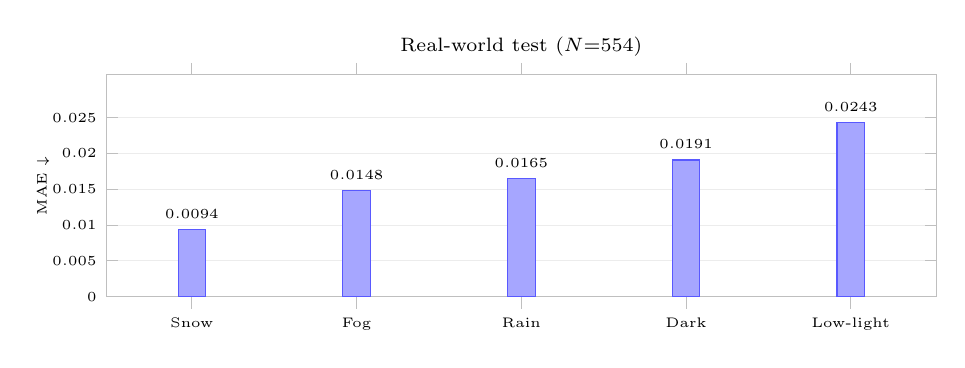
\begin{tikzpicture}
\begin{axis}[
  ybar,
  bar width=10pt,
  width=\columnwidth,
  height=44mm,
  title={Real-world test ($N{=}554$)},
  title style={font=\scriptsize, yshift=-1mm},
  ylabel={MAE $\downarrow$},
  ylabel style={font=\tiny, yshift=-2mm},
  symbolic x coords={Snow, Fog, Rain, Dark, Low-light},
  xtick=data,
  xticklabels={Snow, Fog, Rain, Dark, Low-light},
  xticklabel style={font=\tiny},
  ytick={0.000,0.005,...,0.025},
  yticklabel style={font=\tiny},
  scaled y ticks=false,
  y tick label style={/pgf/number format/fixed, /pgf/number format/precision=3},
  ymin=0, ymax=0.031,
  ymajorgrids=true,
  grid style={gray!15},
  axis line style={gray!50, line width=0.4pt},
  tick style={gray!50, line width=0.4pt},
  nodes near coords,
  every node near coord/.append style={font=\tiny, /pgf/number format/fixed, /pgf/number format/precision=4, anchor=south, yshift=0.5pt},
  enlarge x limits=0.13,
]
\addplot[fill=blue!35, draw=blue!65, line width=0.4pt] coordinates {
  (Snow,      0.0094)
  (Fog,       0.0148)
  (Rain,      0.0165)
  (Dark,      0.0191)
  (Low-light, 0.0243)
};
\end{axis}
\end{tikzpicture}
\caption{\textbf{Weather-wise MAE on real-world test.}
Snow yields the lowest error, while low-light yields the highest.}
\label{fig:weather}
\end{figure}

\begin{table}[t]
\centering
\caption{Weather-wise results on real-world test (554 images).}
\label{tab:weather}
\small
\begin{tabular}{@{}lccccc@{}}
\toprule
Weather & $N$ & MAE $\downarrow$ & $S_\phi$ $\uparrow$ & $F_\beta^{\max}$ $\uparrow$ \\
\midrule
Snow      & 90  & 0.0094 & 0.9478 & 0.9421 \\
Fog       & 126 & 0.0148 & 0.9179 & 0.8914 \\
Rain      & 120 & 0.0165 & 0.9157 & 0.8935 \\
Dark      & 125 & 0.0191 & 0.9072 & 0.8885 \\
Low-light & 93  & 0.0243 & 0.8897 & 0.8629 \\
\bottomrule
\end{tabular}
\end{table}

\subsection{Routing Entropy}
Table~\ref{tab:entropy} reports mean normalized entropy per scale.
Mean normalized entropy ranges from 0.68 to 0.69 across scales, indicating moderate routing uncertainty.
Scale $1/16$ exhibits marginally lower entropy ($0.680$--$0.682$) than scales $1/4$ ($0.691$) and $1/8$ ($0.693$), although the difference is small.
The difference between synthetic and real entropy is less than 0.003 at all scales, indicating similar mean routing entropy across the two test splits.

\begin{table}[h]
\centering
\caption{Mean routing entropy (normalized by $\log 2$).}
\label{tab:entropy}
\small
\begin{tabular}{@{}lcc@{}}
\toprule
Scale & Synthetic & Real \\
\midrule
$1/4$  & 0.6910 & 0.6912 \\
$1/8$  & 0.6931 & 0.6931 \\
$1/16$ & 0.6800 & 0.6822 \\
\bottomrule
\end{tabular}
\end{table}

\subsection{Forced-Expert Analysis}
To probe whether routing provides meaningful specialization, we forced all tokens at scale $1/4$ to expert 0 (bypassing the router), while scales $1/8$ and $1/16$ remained routed normally.
On real-world test: MAE increased by $+0.0002$ ($+0.9\%$), $S_\phi$ decreased by $-0.0012$ ($-0.1\%$).
This marginal degradation admits two interpretations: (a)~the 8-expert pool is over-parameterized for the task, and a single expert can handle most tokens; or (b)~experts have learned similar representations, so bypassing routing has limited impact.
Since only 1 of 3 scales was affected, the full effect of disabling all routing remains unknown.
This result should not be interpreted as evidence for or against routing utility; a complete ablation disabling all three routers simultaneously would be needed.

\subsection{Discussion}
The model demonstrates that spatial token-level routing is feasible for single-RGB SOD without weather-specific supervision.
However, several important limitations must be noted.
First, no controlled comparison against existing methods (NIFM) has been performed; the reported results establish a baseline but do not demonstrate state-of-the-art performance.
Second, the model was trained once without replicate runs, so variance estimates are unavailable.
Third, the forced-expert analysis suggests that expert specialization may be limited, and the benefit of multi-expert routing over a single larger expert remains unclear.
Fourth, the routing entropy values are moderate but their relationship to prediction quality is correlational---we have not established that high-entropy tokens are systematically harder or that the entropy feature improves decoder performance compared to a baseline without it.

\section{Conclusion}

We presented SpatialMoE-SOD, which routes individual spatial tokens to separate expert networks at three independent pyramid scales via context-aware routers, without any weather-specific supervision.
Per-token routing entropy is normalized and injected as an explicit decoder feature via learnable additive fusion.
On WXSOD, the model achieves MAE $0.0192$ (synthetic, 1,500 images) and $0.0168$ (real-world, 554 images), with weather-wise MAE ranging from $0.0094$ (snow) to $0.0243$ (low-light).

Several limitations warrant future investigation.
The model was trained once without replicate runs, so variance estimates are unavailable.
No controlled comparison against existing methods (NIFM~\cite{nifm2025}) has been performed.
The forced-expert analysis suggests limited differentiation among experts at scale $1/4$, and the contribution of the entropy fusion mechanism relative to a baseline without it has not been ablated.
The routing entropy values are moderate ($0.68$--$0.69$) but their causal relationship to prediction quality remains unestablished.
Future work should complete the ablation matrix (routing entropy, number of experts, $K$ value, scale independence), perform head-to-head comparison with existing methods, and analyze per-expert feature specialization via activation visualization.

\balance
\bibliographystyle{ieeetr}
\bibliography{references}

% ============================================================
%  FIGURE 4 -- QUALITATIVE RESULTS
%  (placed after the references so it appears last in the
%   document, on the same final page as the tail of the
%   reference list)
% ============================================================
\vspace{4mm}
\begin{figure*}[b]
\centering
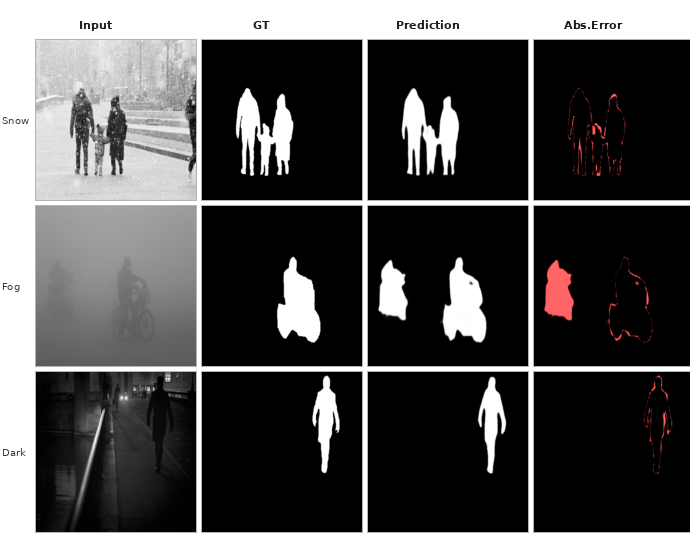
\includegraphics[width=0.75\textwidth]{fig_qualitative.png}
\caption{\textbf{Qualitative results on real-world WXSOD test.}
Three examples spanning snow, fog, and dark conditions.
The error map (rightmost column, red) highlights spatial regions where the prediction deviates from ground truth; larger errors concentrate at object boundaries and in regions with degraded visibility.}
\label{fig:qualitative}
\end{figure*}

\end{document}
